
\includegraphics[height=1.25cm]{images/pictograms/FEM}

\includegraphics[height=1.25cm]{images/pictograms/benchmark}

\includegraphics[height=1.25cm]{images/pictograms/3d}

%%%%%%%%%%%%%%%%%%%%%%%%%%%%%%%%%%%%%%%%%%%%%%%%%%%%%%%%%%%%%%%%%%%%%%%%%%%%%%%%%%%%%%%%%%%%

%\lstinputlisting[language=bash,basicstyle=\small]{python_codes/fieldstone_17/keywords.ascii}

\begin{center}
\inpython
{\small Code: \url{https://github.com/cedrict/fieldstone/tree/master/python_codes/fieldstone_17}}
\end{center}

\par\noindent\rule{\textwidth}{0.4pt}

Last revision: August 14th, 2025.

\par\noindent\rule{\textwidth}{0.4pt}

%%%%%%%%%%%%%%%%%%%%%%%%%%%%%%%%%%%%%%%%%%%%%%%%%%%%%%%%%%%%%%%%%%%%%%%%%%%%%%%%%%%%%%%%%%%%%%%%%%%


This benchmark begins by postulating a polynomial solution to the 3D Stokes 
equation (see \textcite{dobo04} (2004)):
\begin{equation}
\vec{\upnu}
=
\left(
\begin{array}{c}
x+x^2+xy+x^3y \\
y + xy + y^2 + x^2 y^2\\
-2z - 3xz - 3yz - 5x^2 yz
\end{array}
\right)
\label{eqburrr}
\end{equation}
and
\begin{equation}
p = xyz + x^3 y^3z - 5/32
\end{equation}
Following \textcite{busa13} (2013), the viscosity
is given by the smoothly varying function
\begin{equation}
\eta(x,y,z)=\exp(1 - \beta(x(1 - x) + y(1 - y) + z(1 - z)))
\end{equation}
The derivations for the rhs are presented in Section~\ref{MMM-mms_db3D}.


%-----------------------------------
\subsection*{Pressure normalisation} 

Because Dirichlet boundary conditions are prescribed on all sides the 
pressure is known up to an arbitrary constant. This constant can be 
determined by (arbitrarily) chosing 
to normalised the pressure field as follows:
\begin{equation}
\int_\Omega p \; d\Omega = 0 \label{constr1}
\end{equation}
This is a single constraint associated to a single Lagrange multiplier $\lambda$ and 
the global Stokes system takes the form 
\[
\left(
\begin{array}{ccc}
\K & \G & 0 \\
\G^T & 0 & {\cal C}\\
0 & {\cal C}^T & 0
\end{array}
\right)
\left(
\begin{array}{c}
V \\ P \\ \lambda
\end{array}
\right)
\]
In this particular case the constraint matrix ${\cal C}$ is a vector and it only acts on the pressure degrees of freedom because
of Eq.(\ref{constr1}). Its exact expression is as follows:
\[
\int_\Omega p \; d\Omega = \sum_e \int_{\Omega_e}  p \; d\Omega 
=\sum_e \int_{\Omega_e}  \sum_{i} N^p_i p_i \; d\Omega  
=\sum_e \sum_i \left( \int_{\Omega_e}  N^p_i \; d\Omega \right)  p_i 
=\sum_e {\cal C}_e \cdot {\bm p}_e
\] 
where ${\bm p}_e$ is the list of pressure dofs of element $e$. The elemental constraint vector contains the 
corresponding pressure basis functions integrated over the element. These elemental constraints are then 
assembled into the vector ${\cal C}$.

Remark: When using $Q_1 \times P_0$ elements, this benchmark fails 
because of the Dirichlet b.c. on all 6 sides and all three components.
However, as we will see, it does work well with $Q_2 \times Q_1$ elements. 

%----------------------------------
\subsection*{About the code}

As it is now the code is not efficient, and prevents us from running 
higher resolution models: each block $\K$, $\G$ is built as a full matrix, 
and later assembled in the global FE matrix which is also defined as a 
full matrix.
Given the fact that we are relying on second order element in 3d, 
this is quite limiting.


%----------------------------------
\subsection*{Constant viscosity}

\begin{center}
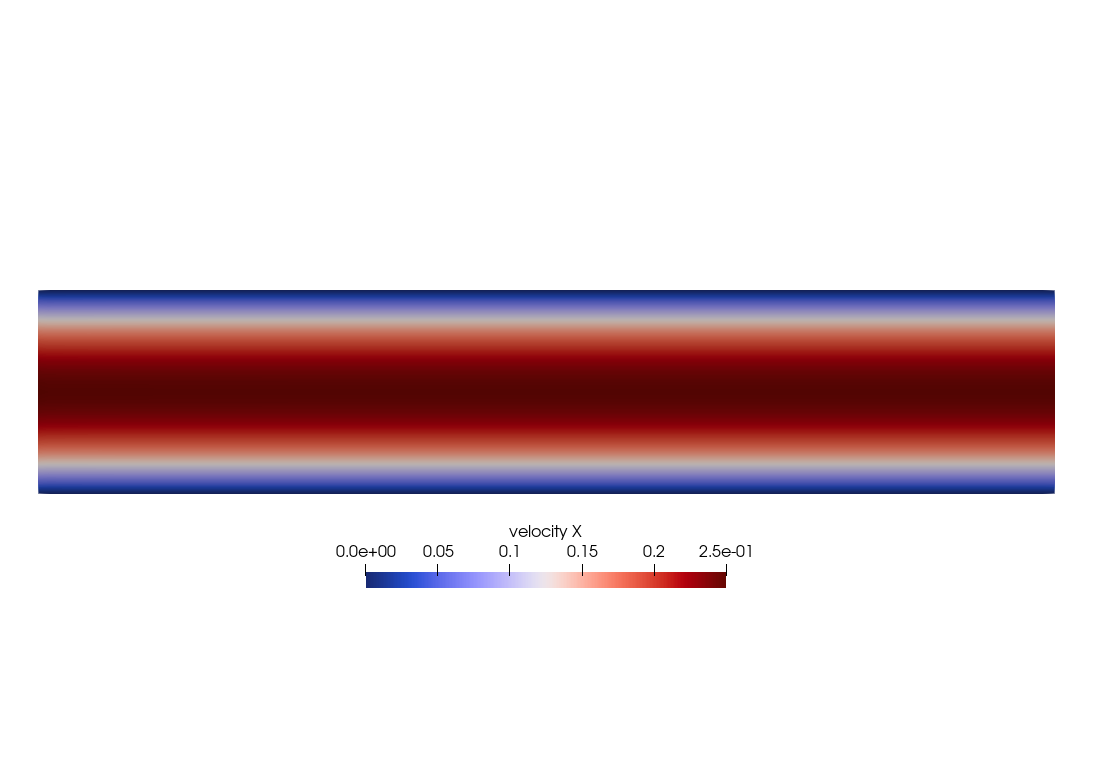
\includegraphics[width=5.6cm]{python_codes/fieldstone_17/results_isoviscous/u}
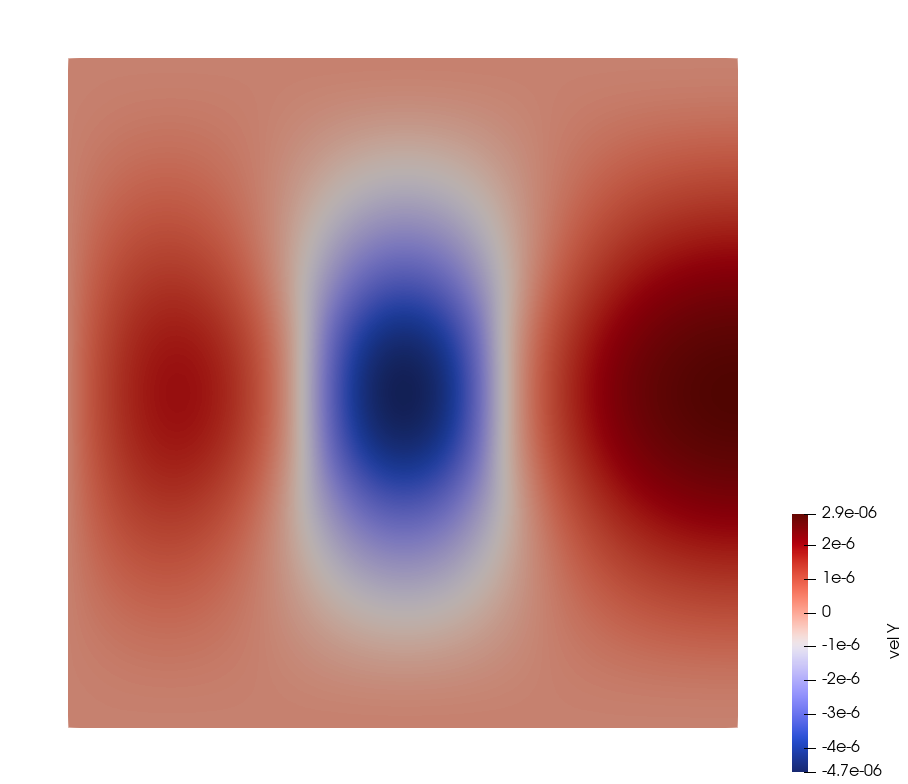
\includegraphics[width=5.6cm]{python_codes/fieldstone_17/results_isoviscous/v}
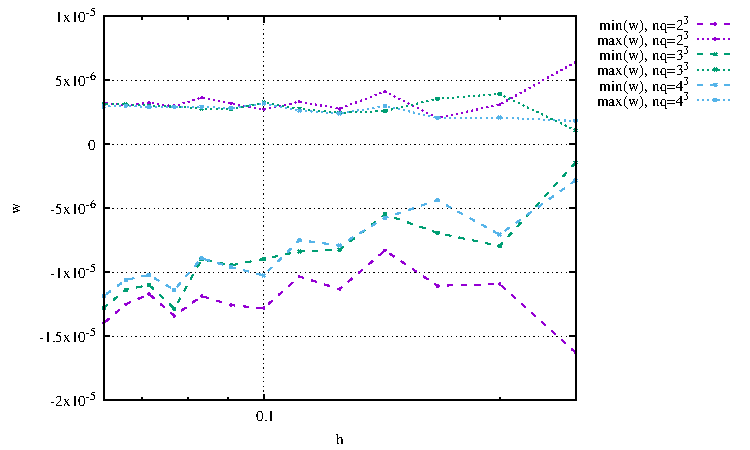
\includegraphics[width=5.6cm]{python_codes/fieldstone_17/results_isoviscous/w}\\
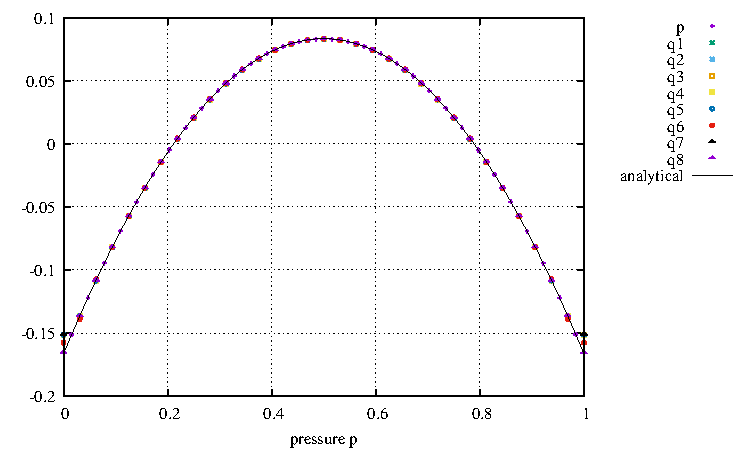
\includegraphics[width=5.6cm]{python_codes/fieldstone_17/results_isoviscous/pressure}
\includegraphics[width=5.6cm]{python_codes/fieldstone_17/results_isoviscous/sr}\\
{\captionfont Velocity, pressure and strain rate fields on a 6x6x6 grid.}
\end{center}

The components of the strain rate tensor are as follows:
\begin{eqnarray}
\dot{\varepsilon}_{xx}&=& 1+2x+y+3x^2y  \nn\\
\dot{\varepsilon}_{yy}&=& 1+x+2y+2x^2y \nn\\
\dot{\varepsilon}_{zz}&=& -2-3x-3y-5x^2y \nn\\
\dot{\varepsilon}_{xy}&=& \frac12 (x+y+2xy^2+x^3) \nn\\
\dot{\varepsilon}_{xz}&=& \frac12( -3z -10xyz ) \nn\\
\dot{\varepsilon}_{yz}&=& \frac12 ( -3z-5x^2z  ) \nn
\end{eqnarray}

The convergence error rates are measured for velocity, pressure and strain rate:
\begin{center}
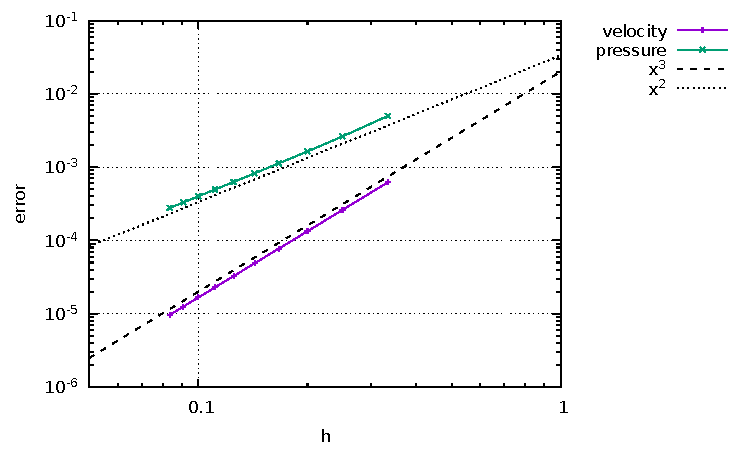
\includegraphics[width=8cm]{python_codes/fieldstone_17/results_isoviscous/errors.pdf}
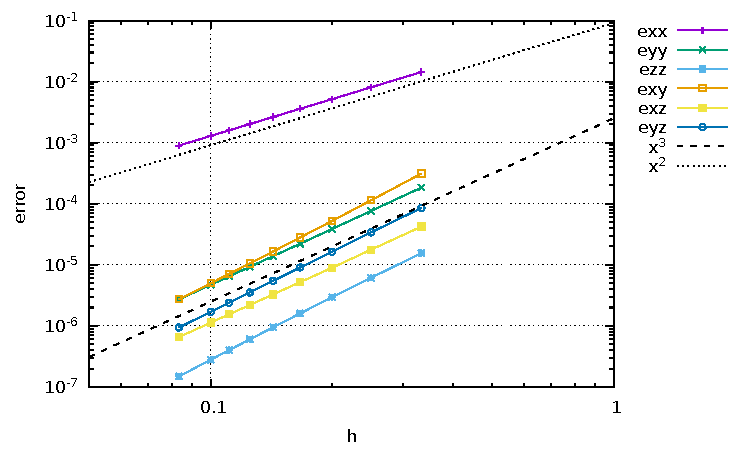
\includegraphics[width=8cm]{python_codes/fieldstone_17/results_isoviscous/errors_sr.pdf}
\end{center}
Since the strain rate is the spatial derivative of the velocity field we should 
find that it converges like $h^2$ as expected. However, since all components of the 
the strain rate are in fact simple/smooth 2nd or 3rd order polynomials the 
recoverred rates are somewhat higher than expected.

I am quite puzzled as to why the convergence 
of $\dot{\varepsilon}_{xx}$ is quadratic 
but at the same time almost 2 orders of magnitude higher than the other 5 components.



%-----------------------------
\subsubsection*{Variable viscosity}

Note that at $(x,y,z)=(0,0,0)$, $\eta=\exp(1)$, 
and at $(x,y,z)=(0.5,0.5,0.5)$, $\eta=\exp(1-3\beta/4)$
so that the maximum 
viscosity ratio is given by 
\[
\eta^\star = \frac{\exp(1-3\beta/4)}{\exp(1)} = \exp(-3\beta/4)
\]
By varying $\beta$ between 1 and 22 we can get up to 7 orders of magnitude viscosity difference.


\begin{center}
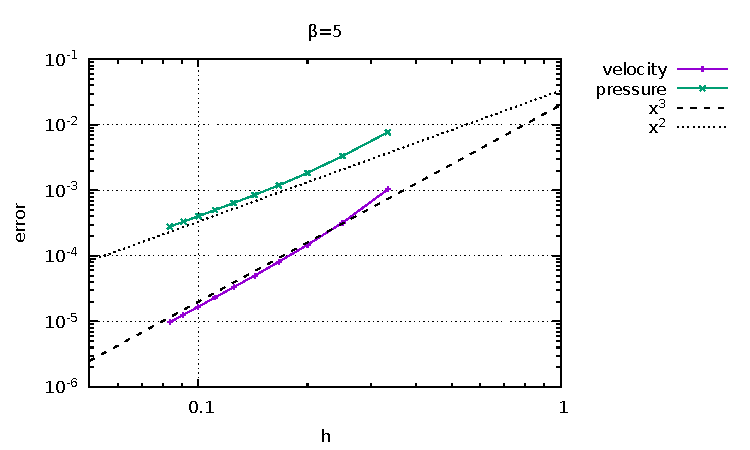
\includegraphics[width=8cm]{python_codes/fieldstone_17/results_beta5/errors.pdf}
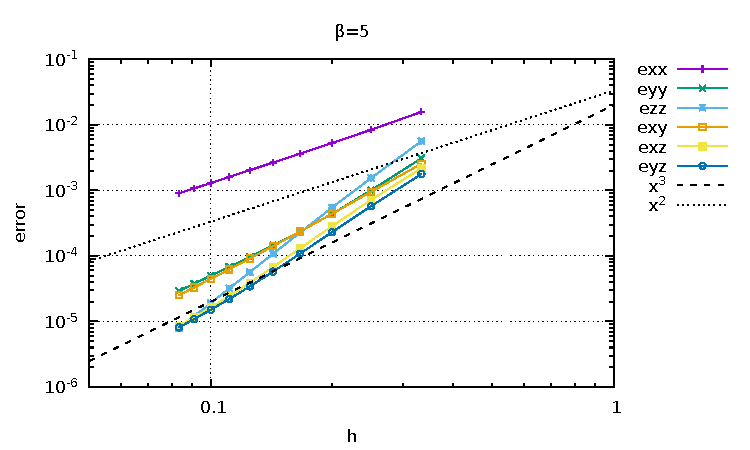
\includegraphics[width=8cm]{python_codes/fieldstone_17/results_beta5/errors_sr.pdf}\\
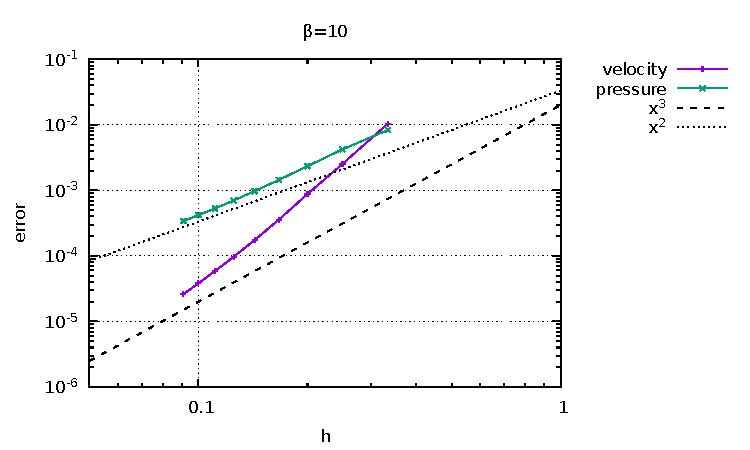
\includegraphics[width=8cm]{python_codes/fieldstone_17/results_beta10/errors.pdf}
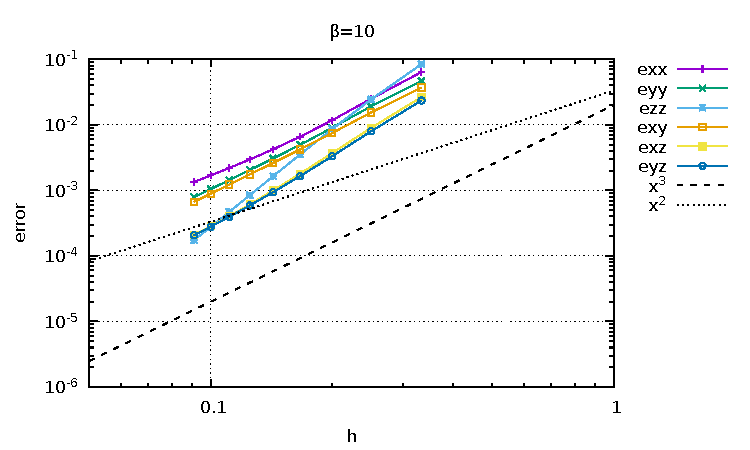
\includegraphics[width=8cm]{python_codes/fieldstone_17/results_beta10/errors_sr.pdf}
\end{center}

We see that with increasing viscosity contrasts higher and higher resolutions are needed to 
attain the expected convergence rates for velocity and pressure. As for strain rate convergence, 
as puzzled as before ...



\begin{center}
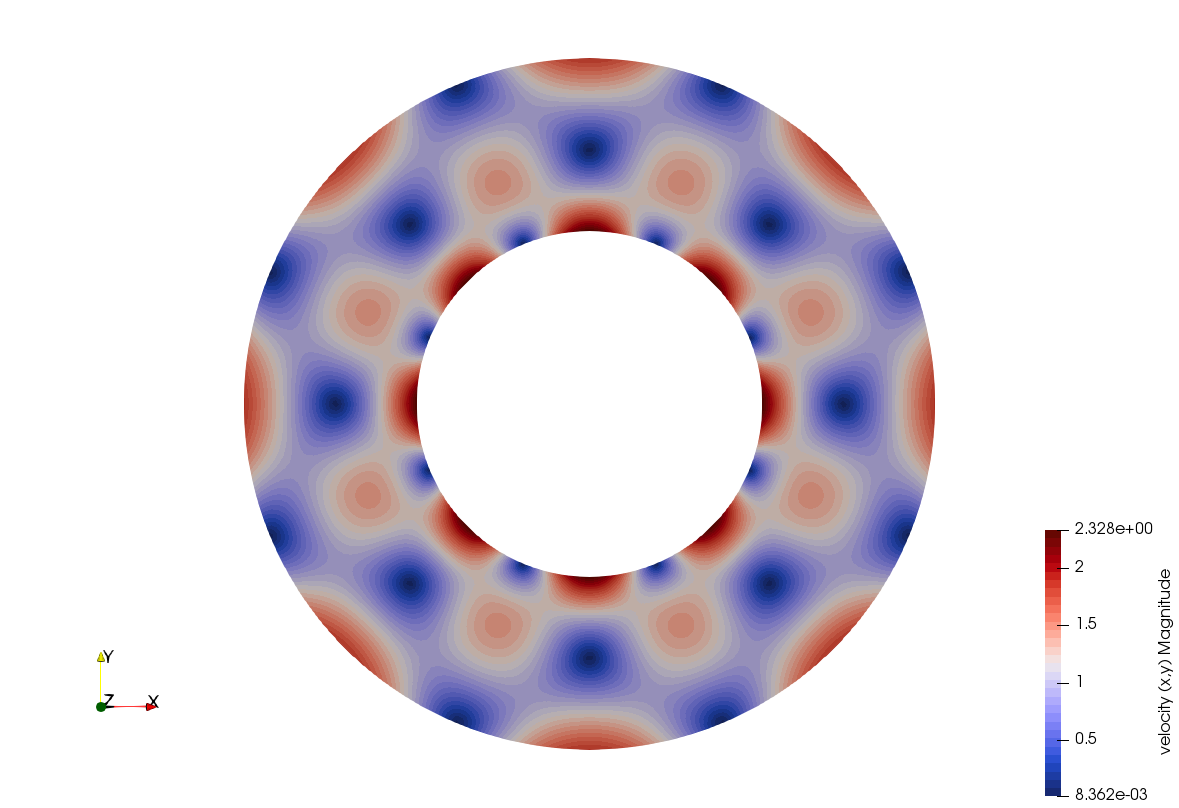
\includegraphics[width=7cm]{python_codes/fieldstone_17/results_beta5/velocity}
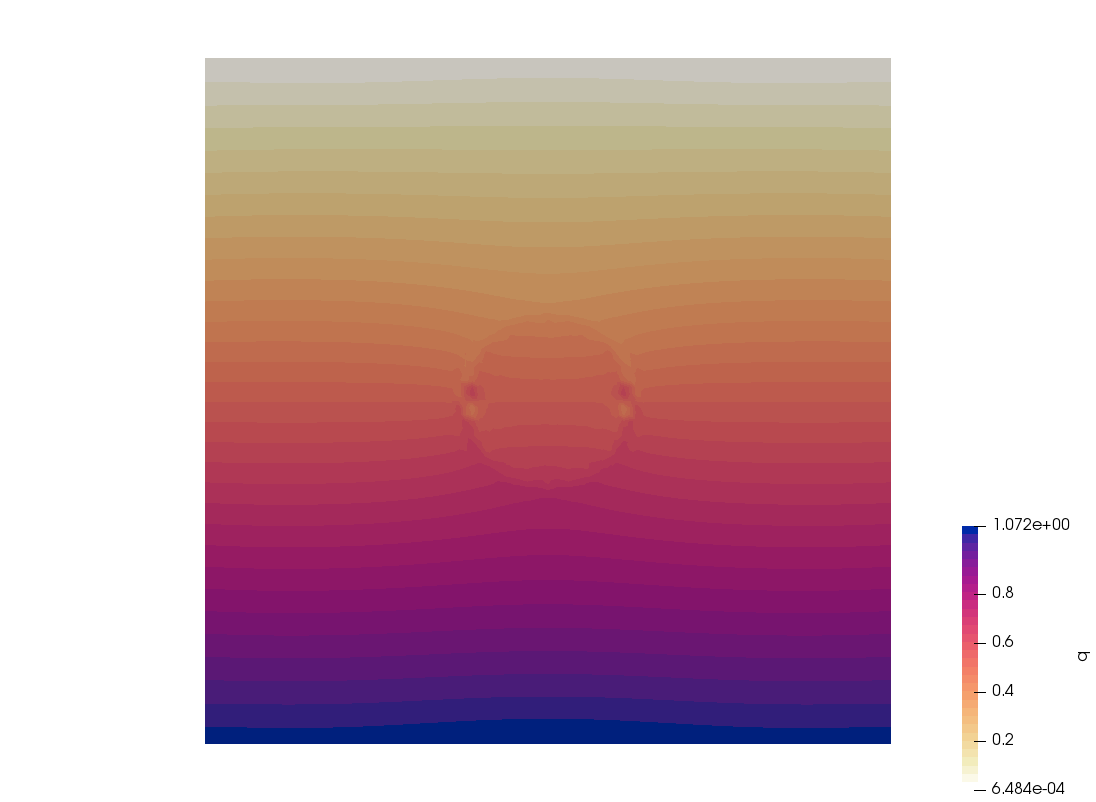
\includegraphics[width=7cm]{python_codes/fieldstone_17/results_beta5/q}\\
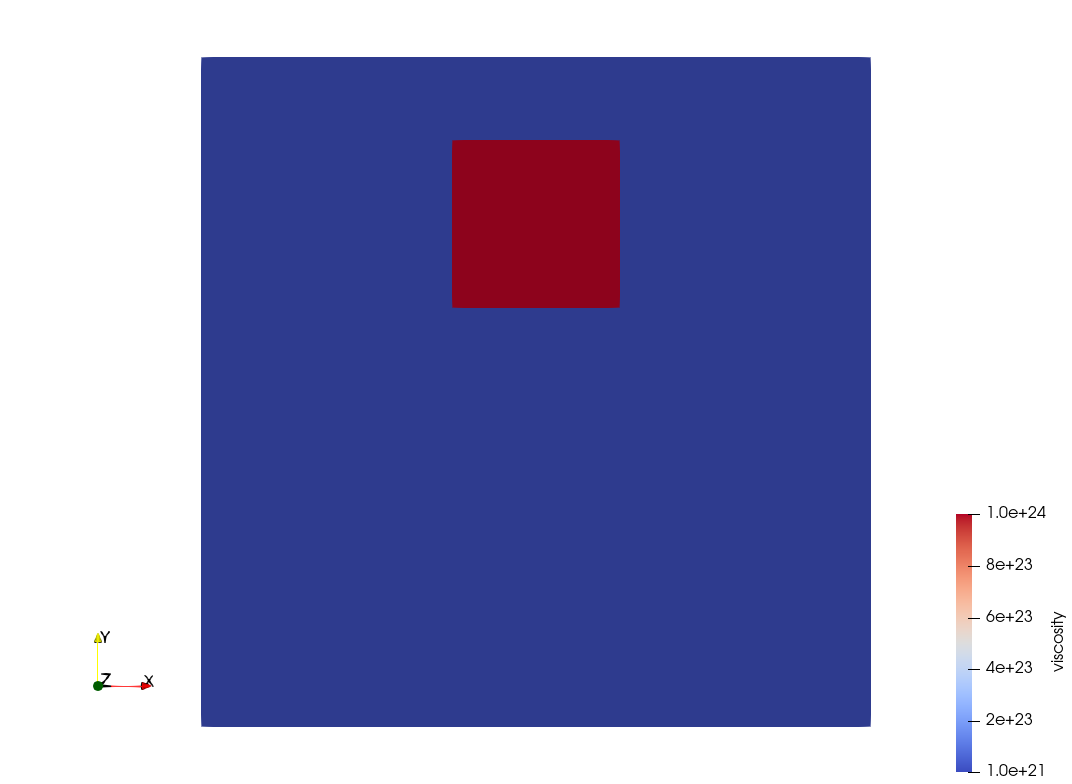
\includegraphics[width=7cm]{python_codes/fieldstone_17/results_beta5/eta}
\includegraphics[width=7cm]{python_codes/fieldstone_17/results_beta5/sr}\\
{\captionfont Obtained for a 10x10x10 mesh and $\beta=5$}
\end{center}

\newpage
%=========================================================================
\section*{ABC flow}

An additional benchmark (also manufactured solution) has been added.
It is described in Section~\ref{MMM-ss:ABCflow}.

\begin{center}
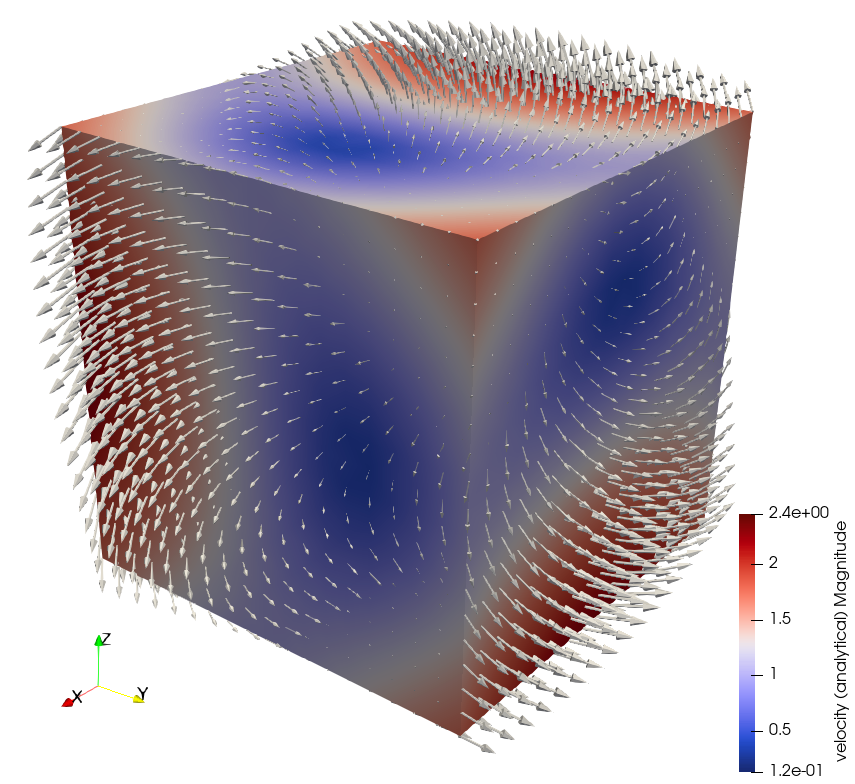
\includegraphics[width=7cm]{python_codes/fieldstone_17/experiment2/vel}
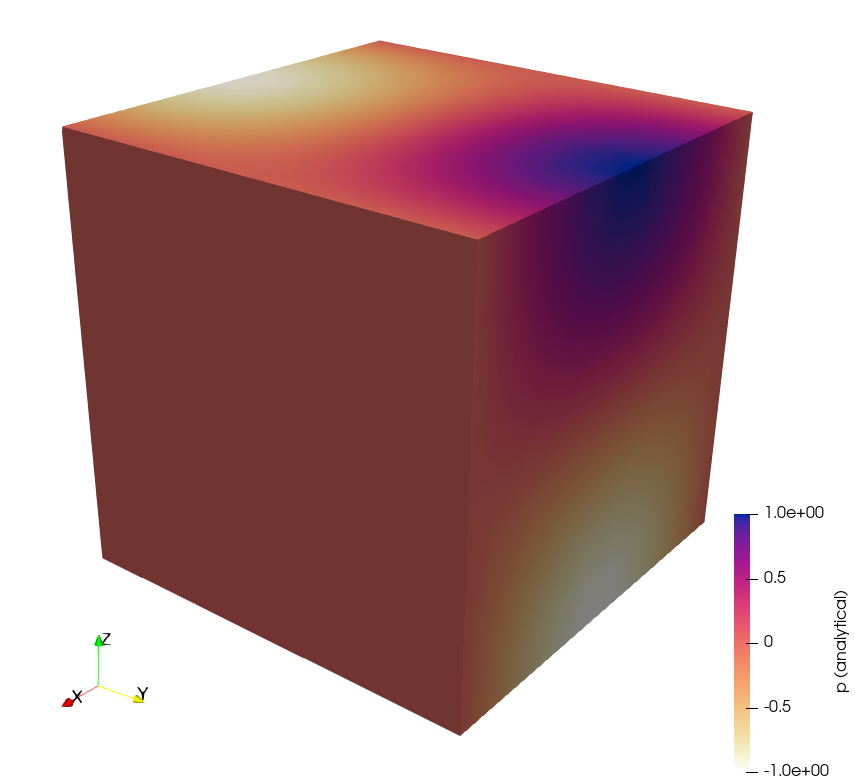
\includegraphics[width=7cm]{python_codes/fieldstone_17/experiment2/press}\\
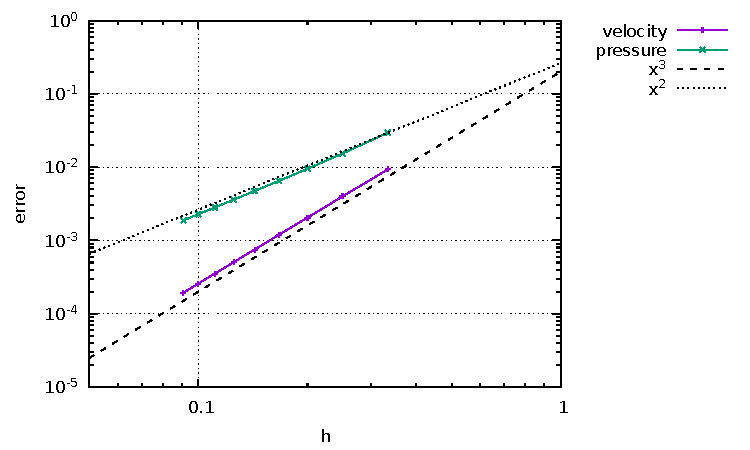
\includegraphics[width=8.2cm]{python_codes/fieldstone_17/experiment2/errors.pdf}
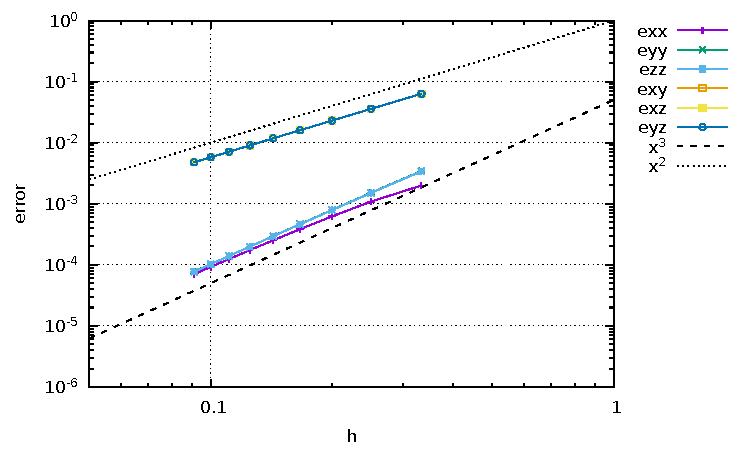
\includegraphics[width=8.2cm]{python_codes/fieldstone_17/experiment2/errors_sr.pdf}
\end{center}














%\begin{center}
%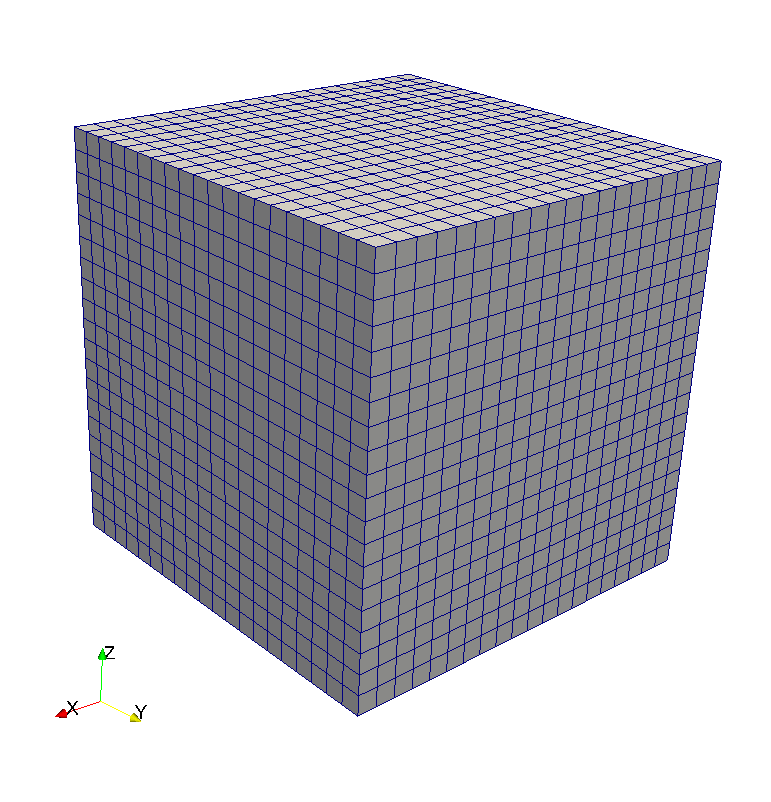
\includegraphics[width=5cm]{python_codes/fieldstone_stokes_sphere_3D/grid}
%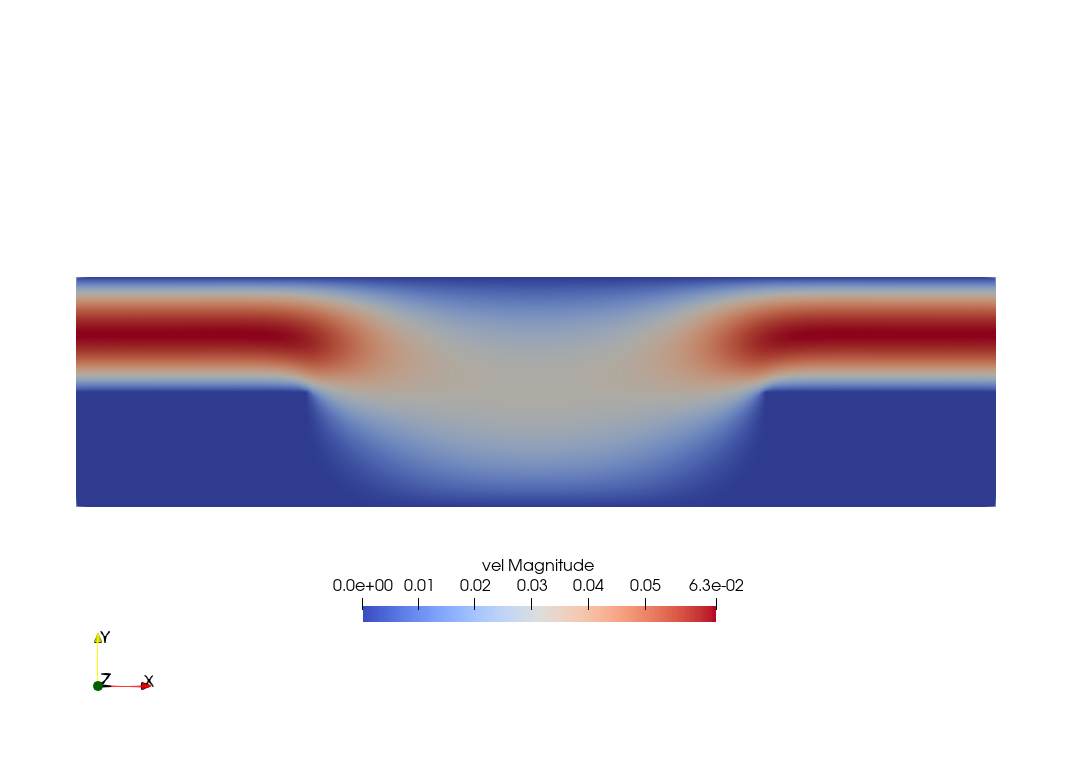
\includegraphics[width=5cm]{python_codes/fieldstone_stokes_sphere_3D/vel}
%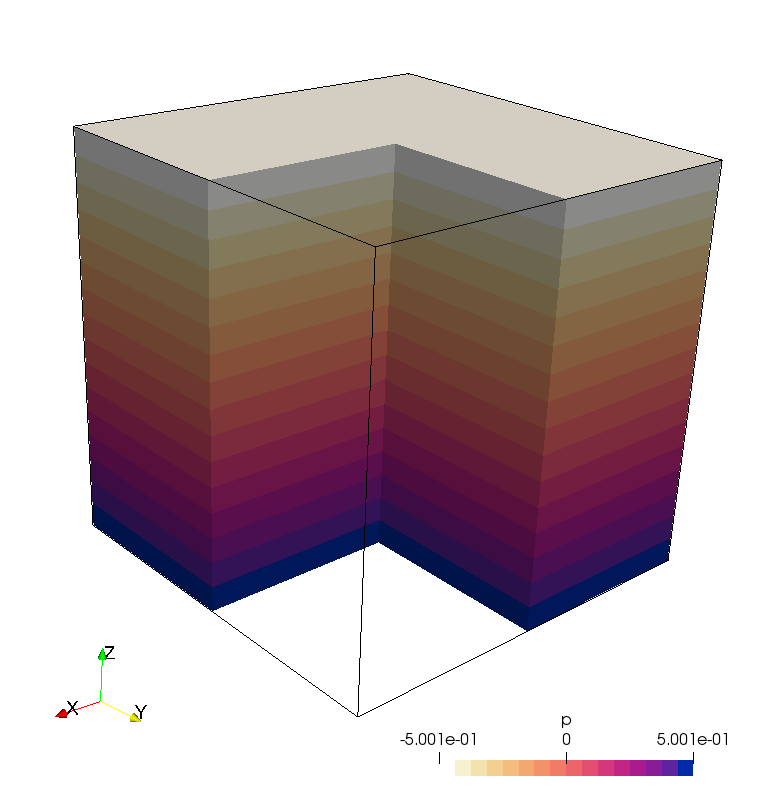
\includegraphics[width=5cm]{python_codes/fieldstone_stokes_sphere_3D/press}\\
%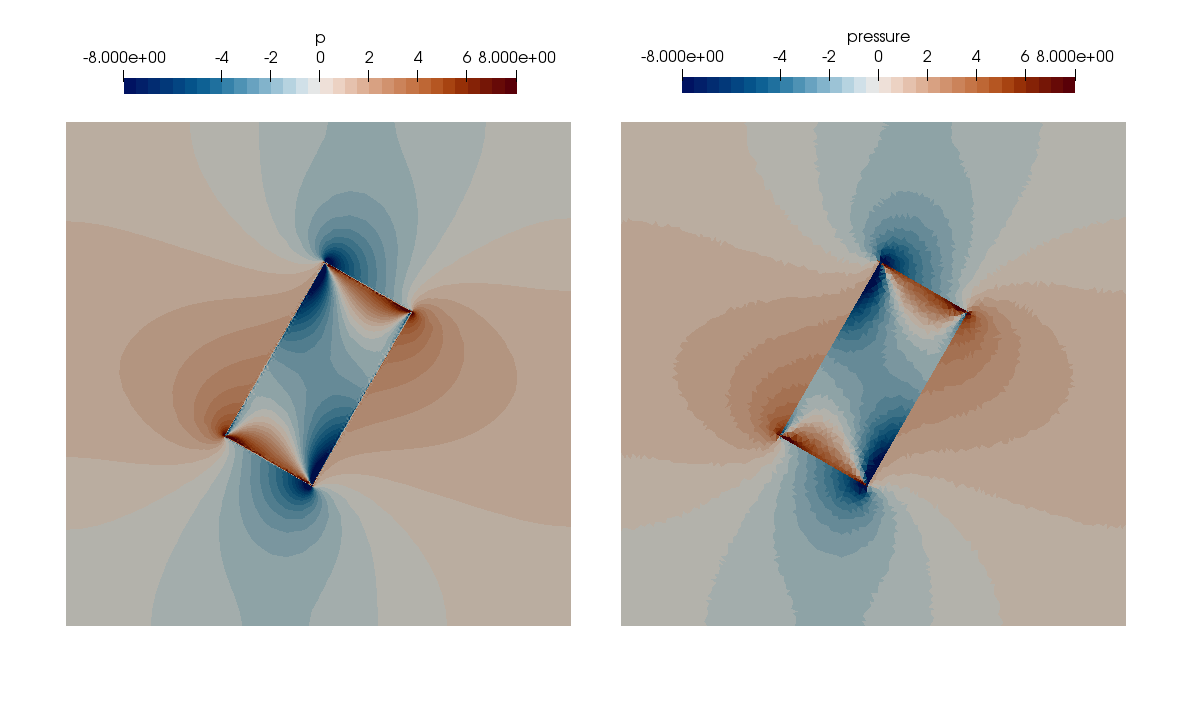
\includegraphics[width=5cm]{python_codes/fieldstone_stokes_sphere_3D/press2}
%\includegraphics[width=5cm]{python_codes/fieldstone_stokes_sphere_3D/visc}
%\includegraphics[width=5cm]{python_codes/fieldstone_stokes_sphere_3D/dens}\\
%{\small resolution is 24x24x24}
%\end{center}

